\documentclass[11pt]{article}
\usepackage{icmlko}
\begin{document}

\title{그 안 재는 도메인은 복도를 옮기고 있었다 --- 문턱은 학습의 1.7\%와 8.5\% 사이}
\author{월드모델 실험실}
\date{노트 362 · 2026년 8월 1일}
\maketitle

\begin{abstract}
\textbf{노트 361을 정정한다.} 그 글은 만화 절반(892행)을 빼도 판이 안
움직이고 전부(1,783행)를 빼야 $+0.0041$ 이 나온다는 것을 보고 ``양이
아니라 있음''이라 적었다. 10\%(178행) 팔을 붙이니 \textbf{$+0.0032$(9/12)}
--- 전부 빼는 것과 거의 같다. \textbf{양이 맞다. 다만 선형이 아니라
문턱이다} --- 178행(학습의 1.7\%)은 0행과 같고 892행(8.5\%)은 1,783행
(17\%)과 같다. 후보 하나는 죽었다: 원핫 열만 빼면 $-0.0018$(\textbf{1/12})로
\emph{나빠진다}. 기제도 찾았다. 만화는 공유 특징 68열 중 \textbf{셋}에서만
다른 도메인과 떨어져 있고(\texttt{venue\_prominence} ·
\texttt{entry\_friction} · \texttt{goods\_scale} 의 \emph{값}), 그 셋에서
\textbf{한쪽 끝에 1,783행이 통째로 쌓여 있다}(\texttt{entry\_friction}
덮음 100\% · 중앙 \textbf{0.00}, 모바일 1.00 · 도서 0.57 · 애니 0.53 대비).
분기의 이득은 그 무리가 손실에서 차지하는 몫에 비례하므로, 17\%일 때는
거기서 가르는 것이 값지고 1.7\%일 때는 후보에도 안 오른다. \textbf{노트
259의 ``복도''가 도메인 크기 축에서 다시 나온 것이고, 이번엔 문턱이
붙었다.}
\end{abstract}

\section{정정 --- 양이 맞다}

\begin{center}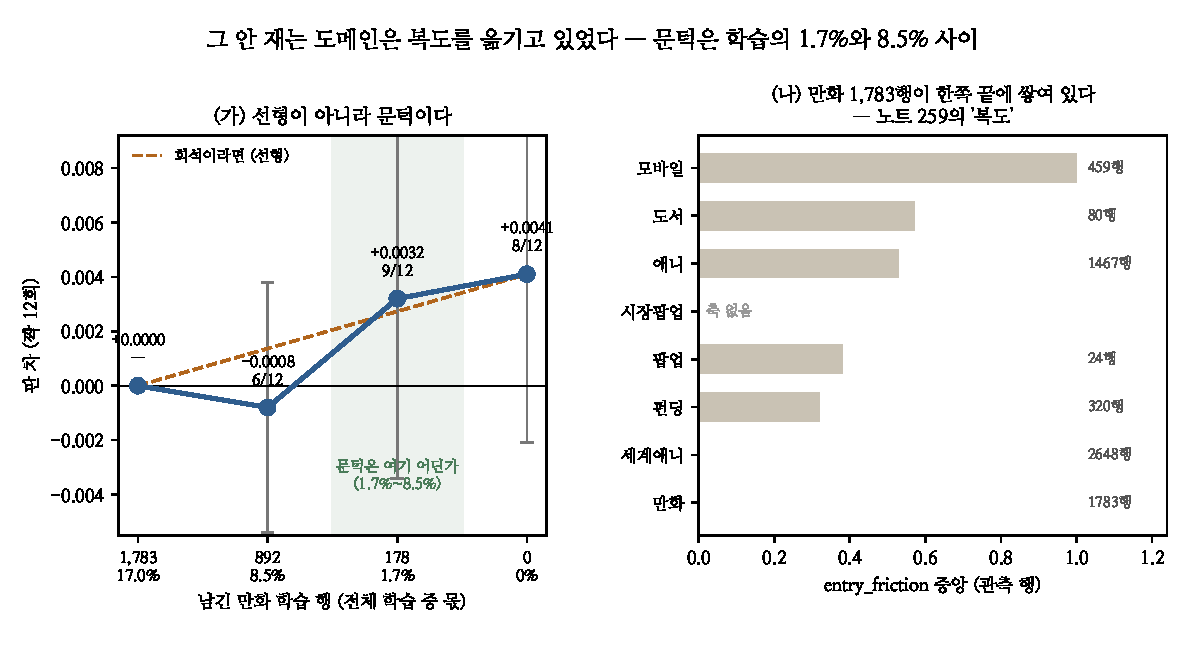
\includegraphics[width=\linewidth]{figs/corridor.pdf}\end{center}

\begin{center}
\begin{tabular}{rrrrl}
\hline
남긴 만화 학습 & 학습 중 몫 & 판 차 & SD & 부호 \\
\hline
1,783 & 17.0\% & --- & --- & --- \\
892   &  8.5\% & $-0.0008$ & 0.0046 & 6/12 \\
\textbf{178} & \textbf{1.7\%} & $\mathbf{+0.0032}$ & 0.0066 & \textbf{9/12} \\
0     &  0\%   & $+0.0041$ & 0.0062 & 8/12 \\
\hline
\end{tabular}
\end{center}

노트 361이 세 점(1,783 · 892 · 0)만 보고 ``있음''이라 읽었다. 네 번째
점이 그 읽기를 뒤집는다 --- \textbf{178행은 없는 것과 같다.} 두 점 사이
어딘가에 문턱이 있고, 그 사이는 학습의 1.7\%에서 8.5\%다.

\textbf{노트 133의 규약이 두 노트 연속으로 일했다.} 361이 첫 답(``있음'')을
그대로 두지 않고 갈래를 걸어 뒀고, 그 갈래가 361을 고쳤다.

\section{원핫은 아니다}

\begin{center}
\begin{tabular}{lrrr}
\hline
 & 판 차 & SD & 부호 \\
\hline
만화 원핫 열만 0 으로 & $-0.0018$ & 0.0017 & \textbf{1/12} \\
\hline
\end{tabular}
\end{center}

행은 그대로 두고 만화의 도메인 지시 열만 죽이면 판이 \emph{내려간다} ---
12번 중 11번이다. 원핫은 범인이 아니라 오히려 일하고 있다(그 열이 있어야
모형이 만화 행을 ``만화라서 그렇다''로 처리하고 지나갈 수 있다).
후보 셋 중 둘이 죽었다(노트 361이 라벨 순위 섞임을, 여기가 원핫을).

\section{남은 하나 --- 자리, 그리고 왜 문턱인가}

만화가 공유 특징 공간에서 어디에 있는지 셌다. 68열 중 중앙값 차가 0.2를
넘는 열은 \textbf{셋뿐}이고(평균 차 0.022 · 중앙 0.000), 셋 다 손 축의
\emph{값} 열이다.

\begin{center}
\begin{tabular}{lrrrr}
\hline
도메인 & 학습 & \texttt{entry\_friction} 덮음 & 중앙 \\
\hline
모바일   & 1,559 & 100\% & 1.00 \\
도서     &    80 & 100\% & 0.57 \\
애니     & 1,467 & 100\% & 0.53 \\
팝업     &    24 &  67\% & 0.38 \\
펀딩     &   320 & 100\% & 0.32 \\
세계애니 & 2,648 & 100\% & 0.00 \\
\textbf{만화} & \textbf{1,783} & \textbf{100\%} & \textbf{0.00} \\
게임 · 시장팝업 · 아이돌 · 웹툰 & --- & 0\% & --- \\
\hline
\end{tabular}
\end{center}

\textbf{만화 1,783행이 이 축의 한쪽 끝에 통째로 쌓여 있다.}
\texttt{venue\_prominence}(만화 중앙 0.00)와
\texttt{goods\_scale}(덮음 68\% · 중앙 0.04)도 같은 모양이다.

\textbf{왜 문턱인가.} 부스팅은 이득이 큰 분기부터 고르고, 어떤 분기의
이득은 그 분기가 가르는 무리가 \emph{손실에서 차지하는 몫}에 대체로
비례한다. 만화가 학습의 17\%면 ``\texttt{entry\_friction} 이 낮다''는
분기가 상위 후보가 되고, 1.7\%면 다른 분기에 밀려 아예 안 뽑힌다.
\textbf{선형이 아니라 켜지고 꺼지는 이유가 이것이다.}

그리고 그 분기가 만들어지면 \emph{다른 도메인의 낮은 행들도 같은 가지로
내려간다}. 세계애니는 중앙이 똑같이 0.00 이고 2,648행이다.
\textbf{노트 259가 잡은 ``복도''와 같은 일이다} --- 그때는 열을 더해서,
여기는 행이 쌓여서 복도가 옮겨진다.

\textbf{칸 나누기는 아니다.} 만화를 1,783 $\to$ 178 로 줄일 때 255분위
경계가 평균 $0.022$ · 최대 $0.070$ 만 움직인다. 부호가 바뀔 크기가 아니다.

\section{그래도 안 넣는다}

10\% 팔은 도메인 여섯을 올린다(펀딩 $+0.0104$ 9/12 · 애니 $+0.0080$ 8/12 ·
웹툰 $+0.0070$ 9/12 · 아이돌 $+0.0260$ 8/12). 그런데 \textbf{팝업이
$-0.0315$(3/12)}다.

노트 275 규칙: 판 $+0.0032$ 는 미결정 폭 안이고, 제일 나쁜 팝업이
$-0.0315/0.0531$ 로 $|t| = 0.59$ 라 문턱 밖이다 $\Rightarrow$ 배포가
정한다 $\Rightarrow$ 팝업이 내려가므로 \textbf{안 넣는다.} 노트 356과
같은 자리, 같은 답이다.

\textbf{세 번째로 같은 모양이다} --- 351(팝업 올라서 넣음) · 356(팝업
내려서 안 뺌) · 362(팝업 내려서 안 넣음). \textbf{판이 미결정 폭 안에서
움직이는 한 이 실험실의 결정은 전부 팝업 65행이 내린다.} 노트 360이
``팝업에 필요한 것은 센 행''이라 적은 이유가 여기에 또 있다.

\section{규약에 더하는 줄}

\begin{itemize}
\item \textbf{용량-반응은 네 점 이상으로 그린다.} 세 점(전부 · 절반 ·
없음)이면 문턱을 있음/없음으로 잘못 읽는다 --- 노트 361이 그랬다.
\item \textbf{채점 안 되는 도메인은 학습 몫으로 관리한다.} 만화는 지금
17\%이고 1.7\%면 해가 사라진다. \emph{빼는 것}과 \emph{줄이는 것}은 다른
선택지다.
\item \textbf{복도는 열로도 행으로도 옮겨진다}(노트 259 확장).
\end{itemize}

\section{남은 것}

\begin{center}
\begin{tabular}{ll}
\hline
갈래 & 지금 아는 것 \\
\hline
문턱이 정확히 어디인가 & 1.7\%\textasciitilde{}8.5\% 사이. 4\% 팔 하나면 좁아진다 \\
다른 도메인도 쌓여 있나 & 세계애니 2,648행도 \texttt{entry\_friction} 중앙 \\
 & 0.00 이다. 같은 검사를 열 도메인에 \\
팝업 실측 41행 & 노트 360. 세 번째 결정도 팝업이 내렸다 \\
만화 2026 스무 건 & 노트 356. 열한 번째 채점 도메인 \\
\hline
\end{tabular}
\end{center}

둘째 줄이 크다. 만화만의 병이 아니라면 \emph{어느 도메인이 어느 축의 끝에
얼마나 쌓여 있나}가 판 전체의 성질이다.

\end{document}
